\documentclass[../main.tex]{subfiles}
\begin{document}
\section{Inventory and Goods}
This section describes the different types of loot and how Characters carry goods in their individual inventories.

\subsection{Goods}
Goods describe anything that can be carried in a Character’s inventory. Fish, materials, and loot all fall under the goods category. Goods can be used on an activated character without energy. For instance,  a character could eat a fish, use loot, and spend material to build during their turn without it costing Energy.

\subsection{Inventory}
Each Character on a team has its own unlimited individual inventory. When a Character performs an action which results in the drawing of a card or collection of a material, that good is placed into the Character’s inventory. 

\begin{figure}[h]
    \centering
    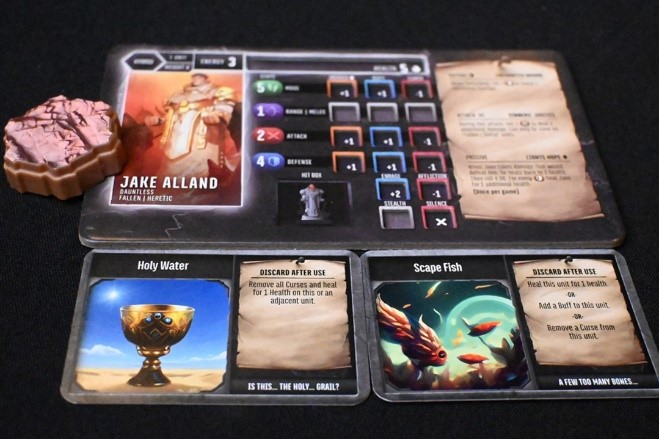
\includegraphics[width=1\linewidth]{chapters//InventoryandGoods/TimeStrikeInventory.jpg}
\end{figure}

\textit{Note: Units who belong to the same multi-unit Character all share the same inventory with one another. To transfer goods between Characters, you can use the Trade Action.}

\textit{Recommendation: We recommend placing goods cards slightly under the Character card to ensure they are associated with that Character, and stacking the material gathered on top of the Character artwork.}

\subsection{Loot}
Loot consists of several different types of cards. Players will discover two different types of loot as they attack the Lost, complete quests, and defeat their enemies.

\subsubsection{Artifacts}
When a Character receives an artifact card, it is placed in their inventory as an unequipped artifact. Unequipped artifacts have no effect. At the start of a Character’s turn, a player may choose to equip one artifact in that Character’s inventory. When a new artifact is equipped, any artifact that was previously equipped to that Character is immediately unequipped. Equipping an artifact is not considered an Action and does not cost any Energy. 

While an artifact is equipped to a Character, it can provide modifiers to their Total Stats, as well as access to powerful new skills or effects.

\begin{figure}[h]
    \centering
    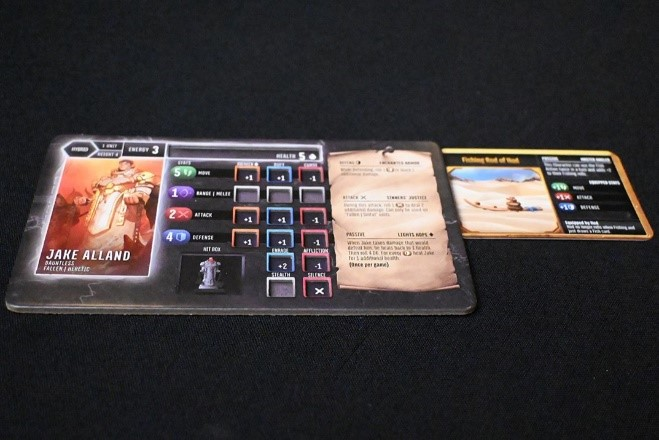
\includegraphics[width=1\linewidth]{chapters//InventoryandGoods/TimeStrikeArtifacts.jpg}
\end{figure}

\textit{Note: Only one artifact can be equipped to a Character at a time.}

\subsubsection{Items}
Items are single-use cards that assist in performing special mechanics that can be exceptions to the default rules of the game. Items can be helpful for attacking, defending, moving, modifying actions, etc.

\clearpage
\end{document}